%%%%%%%%%%%%%%%%%%%%%%%%%%%%%%%%%%%%%%%%%%%%%%%%%%%%%%%%%%%%%%%%%%%%%%
% Evolução da Qualidade Estrutural de Projetos Spring
% TCC - Engenharia de Software - PUC Minas
%
% Para compilar:
%   pdflatex Article.tex
%   bibtex   Article
%   pdflatex Article.tex
%   pdflatex Article.tex
%
% Observação: o arquivo de estilo `sbc-template.sty` deve estar no mesmo
% diretório (download em [https://www.sbc.org.br/documentos-da-sbc/](https://www.sbc.org.br/documentos-da-sbc/)
% summary/169-templates-para-artigos-e-capitulos-de-livros/878-modelosparapublicaodeartigos).
%%%%%%%%%%%%%%%%%%%%%%%%%%%%%%%%%%%%%%%%%%%%%%%%%%%%%%%%%%%%%%%%%%%%%%

\documentclass[12pt]{article}

\usepackage{sbc-template}
\usepackage{graphicx,url}
\usepackage{float}
\usepackage[brazil]{babel}
\usepackage{tabularx}
\newcolumntype{C}{>{\centering\arraybackslash}X}
\usepackage[utf8]{inputenc}
\usepackage[T1]{fontenc}
\usepackage[inline]{enumitem}
\usepackage{tcolorbox}
\usepackage{tikz}
\usetikzlibrary{arrows.meta,positioning}
\usepackage{amsmath}

%%%%%%%%%%%%%%%%% Pacotes para inserção de algoritmos - BEGIN
\usepackage{xcolor}
\definecolor{verde}{rgb}{0.25,0.5,0.35}
\definecolor{jpurple}{rgb}{0.5,0,0.35}
\definecolor{darkgreen}{rgb}{0.0, 0.2, 0.13}

\usepackage{listings}
\lstset{
    language=Java,
    basicstyle=\ttfamily\small,
    keywordstyle=\color{jpurple}\bfseries,
    stringstyle=\color{red},
    commentstyle=\color{verde},
    morecomment=[s][\color{blue}]{/**}{*/},
    extendedchars=true,
    showspaces=false,
    showstringspaces=false,
    numbers=left,
    numberstyle=\tiny,
    breaklines=true,
    backgroundcolor=\color{white!10},
    breakautoindent=true,
    captionpos=b,
    xleftmargin=0pt,
    tabsize=2
}
%%%%%%%%%%%%%%%%% Pacotes para inserção de algoritmos - END

\graphicspath{%
  {imgs/}%
  {Sections/imgs/}%
  {../Divulgacao/Apresentacao/imgs/}%
  {./}%
}

\sloppy

\title{Evolução da Qualidade Estrutural de Projetos Spring:\\transição para Spring Boot e assistência por IA}

\author{Gabriel Ferreira\inst{1}, Guilherme Augusto\inst{1}}

\address{Engenharia de Software\\
  Pontifícia Universidade Católica de Minas Gerais (PUC-MG)\\
  Belo Horizonte -- MG -- Brazil
  \email{\{gabriel.amaral.1447804,gajsouza\}@sga.pucminas.br}
}

\begin{document}

\maketitle

\begin{abstract}
Internal software quality can be described through structural measures of coupling, complexity, inheritance, cohesion and size. This observational longitudinal study follows public Java projects in the Spring ecosystem, focusing on repositories created between 2009 and 2013. Annual snapshots from 2009 to 2025, plus a separately reported partial observation in 2026, are recovered from pinned Git histories. A reproducible sample includes traditional Spring and Spring Boot projects, retaining accessible inactive and archived repositories. Seven measures are extracted with an audited CK instrument. Within-project trajectories and changes surrounding the first observable presence of Spring Boot and AI-assistance evidence are described separately from differences between projects. The analysis reports coverage, medians and paired changes, without interpreting temporal sequence as causation or absence of AI traces as non-use. The frozen sample contains 1,616 candidates; 388 projects contribute 2,533 eligible annual observations. In the oldest cohort, 16 complete-year Boot pairs and only one AI pair are available, plus ten partial-year AI pairs. The dimensions move in different directions, without establishing uniform improvement.
\end{abstract}

\begin{resumo}
A qualidade interna de \emph{software} pode ser descrita por medidas estruturais de acoplamento, complexidade, herança, coesão e tamanho. Este estudo observacional longitudinal acompanha projetos Java públicos do ecossistema Spring, com foco nos repositórios criados entre 2009 e 2013. Recuperam-se versões anuais de 2009 a 2025 e uma observação parcial de 2026, apresentada separadamente, a partir de históricos Git com referências fixadas. A amostra reproduzível inclui Spring tradicional e Spring Boot e mantém projetos inativos e arquivados acessíveis. Sete medidas são extraídas por um instrumento CK auditado. As trajetórias e diferenças dentro de cada projeto, em torno da primeira presença observável de Boot e de evidências de assistência por IA, são separadas das diferenças entre projetos. A análise apresenta cobertura, medianas e mudanças pareadas, sem interpretar sequência temporal como causalidade ou ausência de vestígios de IA como ausência de uso. A amostra congelada contém 1.616 candidatos; 388 projetos contribuem com 2.533 observações anuais elegíveis. Na coorte antiga, há 16 pares completos de Boot e apenas um de IA, além de dez pares parciais de IA. As dimensões se movem em direções distintas, sem estabelecer melhoria uniforme.
\end{resumo}

\begin{tcolorbox}
\footnotesize
\textbf{Bacharelado em Engenharia de \emph{Software} - PUC Minas\\
Trabalho de Conclusão de Curso (TCC)} \\

\indent Orientador de conteúdo (TCC I): Danilo Maia - danilomaia@pucminas.br \\
Orientador de conteúdo (TCC I): João Pedro Batisteli - joaobatisteli@pucminas.br\\
Orientador de conteúdo (TCC I): Leonardo Vilela - leonardocardoso@pucminas.br \\
Orientador acadêmico (TCC I): Cleiton Tavares - cleitontavares@pucminas.br \\
Orientador do TCC II: (A ser definido no próximo semestre)\\ \\
Belo Horizonte, versão de trabalho de 11 de outubro de 2026.
\end{tcolorbox}

\section{Introdução}
\label{sec:introducao}

A qualidade interna de \emph{software} descreve propriedades estruturais do código-fonte, como modularidade, coesão e acoplamento, que podem ser investigadas por análise estática \cite{iso25010,pressman:21}. Em sistemas orientados a objetos, a suíte de Chidamber e Kemerer oferece indicadores para caracterizar essas dimensões \cite{chidamber:94}. Esses indicadores não constituem, isoladamente, uma nota de maturidade: sua interpretação depende do tamanho, do domínio e da organização do projeto.

O ecossistema Spring permite investigar a evolução de projetos Java ao longo de diferentes períodos tecnológicos. Projetos iniciados antes da consolidação do Spring Boot podem ter atravessado mudanças de configuração, dependências, práticas de desenvolvimento e ferramentas de assistência. O Spring Boot 1.0 estável foi lançado em 1º de abril de 2014 \cite{springboot:2014}; por isso, o período de 2009 a 2013 é tratado como contexto de Spring tradicional, com identificação explícita de eventuais versões preliminares de Boot. A presença atual de Boot em um repositório criado em 2010 não demonstra que essa tecnologia já integrava seu código em 2010.

A mesma distinção é necessária para a inteligência artificial. Um projeto antigo pode apresentar hoje vestígios de ferramentas de IA introduzidos recentemente. Datas de criação dos repositórios não datam o uso dessas ferramentas, e fronteiras de calendário não separam perfeitamente produção humana e assistida. O Copilot já estava em prévia técnica em junho de 2021 \cite{copilot:2021}. Evidências de arquivos, identidades e mensagens de commit permitem observar parte dessa adoção, mas não todo uso nem a proporção do código produzida por IA \cite{robbes:26}.

A pergunta central deste trabalho é: \textbf{como a qualidade estrutural de projetos do ecossistema Spring evoluiu ao longo do tempo, e quais mudanças acompanharam a adoção do Spring Boot e o aparecimento de evidências de assistência por IA?} O foco está no acompanhamento dos mesmos projetos, especialmente aqueles criados entre 2009 e 2013. As demais coortes oferecem contexto sobre projetos surgidos em épocas posteriores. Esse desenho distingue evolução dentro do projeto de diferenças de composição entre conjuntos de projetos.

O objetivo geral é descrever longitudinalmente essa evolução por versões anuais recuperadas do histórico Git. Os objetivos específicos são: (i) caracterizar trajetórias de acoplamento, complexidade, tamanho, herança e coesão; (ii) descrever mudanças nos mesmos projetos em torno da primeira presença observável de Spring Boot; (iii) descrever mudanças em torno do aparecimento de evidências de IA; e (iv) comparar essas trajetórias com o contexto de projetos sem a mesma transição observada, considerando tamanho, idade e configuração do framework. O paradigma GQM liga essas perguntas às sete medidas do instrumento CK.

A relevância do estudo está em produzir evidências históricas rastreáveis, com código, datas, versões e cobertura associados a cada medição. A mineração de repositórios possibilita esse acompanhamento, mas exige cuidado com seleção, disponibilidade do histórico e interpretação dos metadados \cite{hassan:08,kalliamvakou:16}. Mudanças de framework, linguagem, domínio, equipe e tamanho são explicações concorrentes para variações das métricas. Nem a injeção de dependências elimina a influência do framework sobre a estrutura, nem um contraste entre períodos permite atribuir diferenças exclusivamente ao desenvolvedor ou à IA.

Os resultados incluem tabelas de cobertura, trajetórias anuais, medianas por época e diferenças entre versões do mesmo projeto, acompanhadas de um pacote de reprodução. A investigação admite estabilidade, aumentos e reduções das métricas, sem presumir melhoria. A Seção~\ref{sec:fund} apresenta a fundamentação; a Seção~\ref{sec:trabalhos}, os trabalhos relacionados; a Seção~\ref{sec:metodologia}, o protocolo histórico; e a Seção~\ref{sec:resultados}, a execução histórica e seus limites, distinguindo-os dos pilotos transversais anteriores.

\section{Fundamentação Teórica}
\label{sec:fund}

Esta seção apresenta os conceitos consolidados que embasam o estudo: qualidade interna de \emph{software}, a suíte de métricas de Chidamber e Kemerer, o paradigma \emph{Goal-Question-Metric}, a mineração de repositórios e a inteligência artificial generativa no recorte da Era da IA assistida.

\subsection{Qualidade interna e métricas orientadas a objetos}
\label{subsec:fund-qualidade}

A norma \emph{ISO/IEC 25010} define qualidade de \emph{software} como um conjunto de características que expressam o grau em que um sistema atende a necessidades explícitas e implícitas \cite{iso25010}. Nesse modelo, a qualidade interna refere-se a propriedades do código-fonte observáveis por análise estática, incluindo modularidade, coesão e facilidade de manutenção. Pressman e Maxim destacam que sistemas com melhor qualidade interna tendem a exigir menor esforço de evolução e a permanecer viáveis por mais tempo \cite{pressman:21}.

Para tornar essas características mensuráveis em código orientado a objetos, Chidamber e Kemerer propuseram um conjunto clássico de indicadores em nível de classe \cite{chidamber:94}. Acoplamento entre objetos (\emph{Coupling Between Objects} --- CBO) descreve o grau de dependência de uma classe em relação a outras. Métodos ponderados por classe (\emph{Weighted Methods per Class} --- WMC) agrega a complexidade dos métodos. Profundidade da árvore de herança (\emph{Depth of Inheritance Tree} --- DIT) e número de filhos (\emph{Number of Children} --- NOC) caracterizam a hierarquia. Resposta de uma classe (\emph{Response for a Class} --- RFC) estima o conjunto de métodos potencialmente acionados a partir de uma mensagem. Falta de coesão em métodos (\emph{Lack of Cohesion in Methods} --- LCOM) indica o quanto os métodos de uma classe operam sobre conjuntos disjuntos de atributos. Essas métricas passaram a ser amplamente empregadas para caracterizar projeto, manutenção e falhas em sistemas orientados a objetos \cite{singh:12,radjenovic:13,aniche:16}. A forma operacional em que serão extraídas neste trabalho, incluindo a ferramenta e as variantes adotadas, é especificada na Seção~\ref{sec:metodologia}.

Neste estudo, WMC representa a complexidade estrutural agregada dos métodos, conforme a implementação do CK; não mede tempo de execução, consumo de recursos ou desempenho computacional. O CBO empregado é o indicador geral de dependências entre classes do CK, sem uma separação implementada entre acoplamento horizontal e vertical. Para coesão, utiliza-se a coluna \texttt{lcom*}, variante normalizada documentada pelo instrumento, e não a coluna \texttt{lcom} original. Valores devem ser interpretados em conjunto: nenhuma métrica isolada prova violação de um princípio de projeto, nem identifica a autoria humana ou assistida do código.

\subsection{Goal-Question-Metric}
\label{subsec:fund-gqm}

O paradigma \emph{Goal-Question-Metric} (GQM) organiza avaliações de \emph{software} em três níveis: o objetivo do estudo (\emph{goal}), as perguntas que o detalham (\emph{questions}) e as métricas que as respondem (\emph{metrics}) \cite{basili:94}. A abordagem evita coletar indicadores sem vínculo com a intenção da pesquisa: primeiro define-se o que se deseja aprender; em seguida, traduz-se esse objetivo em perguntas mensuráveis; por fim, escolhem-se as medidas adequadas. Neste trabalho, o GQM liga o objetivo de analisar a evolução da qualidade estrutural em projetos do ecossistema Spring às dimensões de acoplamento, complexidade, herança, coesão e tamanho, operacionalizadas na Seção~\ref{sec:metodologia}.

\subsection{Mineração de Repositórios de Software}
\label{subsec:fund-msr}

A Mineração de Repositórios de \emph{Software} (\emph{Mining Software Repositories} --- MSR) analisa artefatos reais --- código-fonte, histórico de versões e metadados de plataformas --- para identificar padrões de desenvolvimento, evolução e qualidade \cite{hassan:08}. Em vez de apoiar-se apenas em relatos ou documentação, a MSR observa evidências extraídas dos próprios repositórios. No GitHub, essa estratégia exige filtros de relevância, exclusão de \emph{forks} e distinção entre criação na plataforma, idade do código e disponibilidade de versões, a fim de evitar a interpretação de metadados atuais como evidência histórica \cite{kalliamvakou:14,kalliamvakou:16}. Esses cuidados conceituais orientam a amostragem descrita na metodologia.

\subsection{Inteligência artificial generativa}
\label{subsec:fund-ia}

Neste trabalho, inteligência artificial generativa designa sistemas baseados em modelos de linguagem de grande escala, treinados em corpora de texto e código, capazes de produzir ou completar trechos de programa a partir de contexto e de \emph{prompts}. Ferramentas como GitHub Copilot, ChatGPT, Claude Code e Cursor ilustram esse paradigma e delimitam o que se denomina Era da IA assistida, adotada como quarta época histórica do estudo. Experimentos controlados indicam ganhos de produtividade e variações na qualidade do código sugerido por esses assistentes \cite{peng:23,dakhel:23}, o que motiva investigar se a estrutura interna de projetos Spring publicados no GitHub apresenta sinais observáveis nesse período.

\section{Trabalhos Relacionados}
\label{sec:trabalhos}

Esta seção discute sete estudos empíricos da engenharia de \emph{software} que tratam da qualidade de código assistido por IA, da corretude de artefatos gerados por modelos de linguagem ou da interpretação de métricas de acoplamento em Java. Para cada trabalho, apresentam-se o objetivo e o método, os resultados pertinentes a este TCC e a relação com a proposta --- complementar, comparar ou reutilizar o mesmo tipo de evidência. Os três primeiros artigos foram publicados em 2023 e estão diretamente ligados ao recorte da Era da IA assistida.

A qualidade do código produzido por assistentes foi avaliada de forma experimental com o conjunto HumanEval, comparando GitHub Copilot, Amazon CodeWhisperer e ChatGPT quanto a validade, correção, segurança, confiabilidade e manutenibilidade \cite{yetistiren:23}. O método consistiu em gerar soluções a partir de enunciados e inspecionar o código resultante com métricas de qualidade e critérios de aceitação dos testes do \emph{benchmark}. Os resultados indicam taxas de correção de 65,2\% para o ChatGPT, 46,3\% para o Copilot e 31,1\% para o CodeWhisperer, além de dívida técnica média associada a \emph{code smells} da ordem de minutos por trecho. Esse estudo é complementar ao presente trabalho: enquanto avalia trechos gerados em tarefas isoladas, esta pesquisa observa a estrutura de repositórios Spring reais ao longo do tempo, permitindo contrastar o período anterior à disseminação de assistentes com a Era da IA assistida.

A capacidade do GitHub Copilot como programador-par foi examinada em dois conjuntos de tarefas: problemas algorítmicos fundamentais e um corpus de soluções humanas, corretas e defeituosas \cite{dakhel:23}. O método combinou geração repetida de soluções, verificação de funcionalidade e comparação com implementações de programadores. Os resultados mostram que o Copilot produz soluções para a maioria dos problemas, porém parte delas é defeituosa ou não reproduzível; a taxa de correção humana superou a do assistente, embora o código gerado com falhas tenda a exigir menor esforço de reparo. Os autores concluem que a ferramenta pode ser um ativo para desenvolvedores experientes e um passivo para novatos. O presente trabalho não replica o desenho de tarefas algorítmicas; em vez disso, complementa essa evidência ao perguntar se a adoção massiva de assistentes, a partir de 2022, coincide com mudanças nas métricas estruturais de projetos Java/Spring Boot publicados no GitHub.

A correção funcional de código gerado por modelos de linguagem, incluindo o ChatGPT, foi avaliada com o \emph{framework} EvalPlus, que amplia o HumanEval com uma quantidade substancialmente maior de casos de teste obtidos por geração automática e mutação \cite{liu:23}. O método consistiu em reexecutar 26 modelos populares sobre HumanEval e HumanEval+, medindo \emph{pass@k}. Os resultados mostram quedas de até 19,3\%--28,9\% em \emph{pass@k} quando os testes adicionais são considerados, e alteração no ranqueamento de modelos --- inclusive casos em que o ChatGPT deixa de superar alternativas de código aberto. A relação com este trabalho é de complementaridade: os resultados de \cite{liu:23} demonstram que a qualidade funcional do código gerado por IA é frequentemente superestimada em \emph{benchmarks} curtos; o presente estudo desloca o foco da correção de funções sintéticas para a qualidade estrutural de sistemas Spring completos, em versões históricas.

O impacto da injeção de dependências sobre a manutenibilidade em projetos Java foi investigado com duas métricas ponderadas --- DCE e DCBO --- implementadas no CKJM-Analyzer, extensão da ferramenta CKJM \cite{sun:22}. O método aplicou análise estática a um conjunto de projetos \emph{open source}, distinguindo acoplamento ``suave'' (via injeção) de acoplamento ``rígido'' (instanciação direta). Os resultados indicam que a injeção de dependências reduz o acoplamento efetivo quando este é ponderado, o que métricas clássicas de CBO tendem a não capturar integralmente. O presente trabalho compartilha o objeto de estudo --- código Java com forte presença de injeção, típica do Spring Boot ---, porém não propõe métricas novas: utiliza a suíte CK de forma consistente entre épocas para observar evolução estrutural, reconhecendo a limitação apontada por \cite{sun:22} na interpretação do acoplamento.

O efeito do GitHub Copilot sobre a produtividade de desenvolvedores profissionais foi medido em experimento controlado, com tarefa de implementação cronometrada e grupo de controle sem o assistente \cite{peng:23}. O método alocou participantes de forma aleatória e comparou tempo de conclusão e taxa de término. Os resultados apontam redução substancial do tempo necessário para completar a tarefa (cerca de 55\% mais rápido no grupo com Copilot) e maior taxa de conclusão. Essa evidência fundamenta a delimitação da quarta época histórica (a partir de 2022) como Era da IA assistida. A diferença em relação a este trabalho é o construto medido: o experimento de \cite{peng:23} avalia desempenho individual em uma tarefa; aqui se avaliam métricas estruturais de repositórios públicos, sem reivindicar causalidade direta entre o uso de um assistente específico e a qualidade de cada projeto.

A identificação automatizada de contas que realizam commits de forma não humana em repositórios públicos foi sistematizada por \cite{dey:20}, que propõem a abordagem BIMAN (\emph{Bot Identification by commit Message, commit Association, and author Name}). O método combina três heurísticas independentes --- análise de padrões no nome e no endereço de correio eletrônico do autor (BIN), medição de repetitividade das mensagens de commit por alinhamento de sequência (BIM) e análise de características estruturais dos commits por floresta aleatória (BICA) --- integradas em um classificador de \emph{ensemble} que obteve AUC-ROC mediano de 0,90. Concebido em 2020, o BIMAN identifica com precisão bots de automação clássicos, como \emph{Dependabot}, bots de integração contínua e sincronizadores de código. Sua principal limitação para o presente trabalho é que ferramentas de IA generativa, como GitHub Copilot e Cursor, frequentemente realizam commits sob as credenciais Git do próprio desenvolvedor, sem criar uma identidade de bot própria, o que torna a análise de nome e de mensagem insuficiente para detectar esse padrão de adoção.

A identificação de vestígios de agentes de codificação foi estudada por \cite{robbes:26}, em uma análise de 128.018 projetos públicos do GitHub. O trabalho distingue agentes com maior autonomia de assistentes de completamento e explora rastros como configuração e coautoria. A versão consultada relata adoção estimada entre 22,20\% e 28,66\% no universo investigado. Esses resultados pertencem ao desenho e ao detector dos autores. O presente TCC utiliza uma adaptação local, com um conjunto próprio de heurísticas e inspeção do histórico Git; sua precisão não é herdada automaticamente daquela publicação. Sinais genéricos ou anteriores à disponibilidade das ferramentas exigem revisão contextual.

Os estudos sobre produtividade e correção de trechos gerados não substituem o acompanhamento estrutural de sistemas completos. O presente trabalho combina medidas CK consistentes com versões anuais, distinguindo a evolução do mesmo projeto das diferenças entre projetos de uma época. O foco inclui a transição de Spring tradicional para Boot, enquanto a IA constitui um marco posterior possível, sem restringir toda a investigação a esse contraste. O desenho histórico e suas limitações são apresentados a seguir.

\section{Materiais e Métodos}
\label{sec:metodologia}

O estudo é empírico, quantitativo, observacional e longitudinal. A unidade de acompanhamento é o repositório; a unidade de medição é uma versão anual de seu código. A análise principal acompanha projetos criados entre 2009 e 2013, e as demais coortes oferecem contexto. As conclusões descrevem mudanças e associações. Uma sequência antes/depois não identifica, por si só, um efeito causal de Spring Boot ou de IA.

\subsection{Ambiente e instrumentos}
\label{subsec:ambiente}

O instrumento \texttt{analisar\_evolucao.py} separa recontagem, descoberta, planejamento, coleta e relatório. A descoberta utiliza a API REST de busca do GitHub, com paginação particionada e controle de limites. Os filtros e o sorteio operam sobre metadados salvos. A clonagem e a inspeção de evidências de IA são posteriores ao congelamento da amostra; a inspeção histórica usa objetos Git locais, sem requisições por snapshot.

A extração reutiliza CK 0.7.1-SNAPSHOT do commit \texttt{8a1ef916d597d33ad619d748b616bb7dbc3f0c36}, com JDT 3.44.0 e o adaptador auditado que preserva a chave arquivo e classe. A JVM, os parâmetros, os hashes do JAR, do adaptador e dos scripts são registrados e congelados. Nenhum projeto amostrado é compilado ou executado, nem suas dependências são baixadas. As fórmulas permanecem as do CK; dependências ausentes e resolução parcial de tipos continuam sendo limitações \cite{aniche:ck,child:19}.

\subsection{Descoberta, filtros e sorteio}
\label{subsec:amostragem}

Reaproveita-se a população original de 95.894 repositórios da consulta \texttt{topic:spring-boot fork:true}, salva antes dos filtros em setembro de 2026. Essa população é unida às consultas por tópicos \texttt{spring}, \texttt{spring-framework} e \texttt{spring-mvc}, com deduplicação pelo identificador do GitHub. A procedência e as datas de observação são preservadas, sem apresentar a união como um censo simultâneo. Tópicos indicam candidatos; a confirmação de Spring ocorre no conteúdo das versões históricas.

Aplicam-se localmente filtros de linguagem principal Java, forks, espelhos, repositórios desabilitados, templates, vazios e materiais claramente não relacionados a desenvolvimento de software. Os critérios operacionais de nomes e tópicos são preservados em configuração, e casos educacionais ambíguos permanecem sinalizados para revisão. Arquivamento e falta de atividade recente não excluem candidatos. Projetos que deixaram de estar acessíveis são registrados como falhas de recuperação, sem substituição silenciosa.

As coortes de criação são E1 (2009--2013), E2 (2014--2017), E3 (2018--2021) e E4 (2022--2026, até o corte da execução). A data de criação estratifica o sorteio; a data do snapshot determina a época de cada medição. Para cada coorte, ordenam-se candidatos pelo SHA-256 de \texttt{20261011:identificador}, selecionando até 500; quando houver menos, incluem-se todos. A semente e a lista são congeladas antes das métricas. Os primeiros dez sorteados de cada coorte formam o piloto, com até 40 candidatos. Não se substituem candidatos por falha, tamanho ou resultado CK. O teto por coorte produz frações amostrais diferentes: as medianas conjuntas descrevem a amostra observada, sem ponderação para estimar a distribuição de toda a população do GitHub.

Depois de fixar a amostra e o piloto, ordena-se o processamento por atividade recente, antiga e data desconhecida. Essa ordem é operacional e não altera pertencimento à amostra. Antes da clonagem, publicam-se população, exclusões e candidatos por coorte, com comprovação de retenção de inativos e arquivados.

\subsection{Recuperação das versões históricas}
\label{subsec:snapshots}

Cada repositório é clonado uma vez com o histórico completo alcançável da branch padrão, sem limite de profundidade ou de 30 commits. A referência e seu SHA são fixados. O histórico é percorrido pelo primeiro pai dos merges, representando a linha principal de integração \cite{git:firstparent}. Para cada encerramento de ano em UTC, seleciona-se o último commit dessa linha com data de committer anterior ou igual ao corte. Registra-se também a data de autoria. A data Git do committer é uma aproximação operacional da integração, não prova de quando o conteúdo foi publicado no GitHub.

Medem-se os anos completos de 2009 a 2025. O ano de 2026 usa o instante fixado no início da execução e é apresentado separadamente como período parcial. Sem novos commits, reutiliza-se o SHA anterior e marca-se ``sem novo commit''. Sem histórico anterior ao corte, registra-se ausência de snapshot. Datas não monotônicas, autoria futura, ancestrais posteriores ao corte e histórico raso ou incompleto geram diagnósticos; nenhum caso é substituído pelo código atual. Históricos anteriores à criação do repositório no GitHub são sinalizados como possíveis importações ou migrações.

Cada observação conserva identificador, ano, corte, SHA, datas, framework, versões declaradas, cobertura, métricas e motivos de exclusão. Extrações idênticas são reutilizadas pelo hash do inventário de fontes Java e do instrumento. As evidências de IA mantêm uma chave temporal própria, pois árvores iguais podem ter históricos distintos. Resultados concluídos são reutilizados na retomada; erros permanecem explícitos.

\subsection{Framework e evidências de assistência por IA}
\label{subsec:identificacao-ia}

A identificação técnica inspeciona declarações Maven e Gradle disponíveis no snapshot, distinguindo dependências de produção, testes, gerenciamento, catálogos e plugins. Referências locais de propriedades e versões são resolvidas quando possível; valores não resolvidos são preservados. Um catálogo sem uso não confirma adoção. Dependências exclusivamente de teste não confirmam Boot no código de produção. Código do próprio framework Spring é identificado separadamente e não integra a comparação principal de projetos que utilizam Spring. Declarações de perfis são registradas como condicionais; a análise estática não confirma a configuração efetivamente executada.

Um complemento de classificação resolve usos efetivos de mapas Groovy em scripts Gradle locais referenciados por \texttt{apply from}, incluindo indireções para catálogos TOML. As declarações são lidas no mesmo SHA; expressões dinâmicas e referências ambíguas permanecem sem resolução. O complemento tem hash próprio, preservando a identificação do produtor CK e seus valores brutos. Essa emenda está identificada na execução derivada, sem ser apresentada como componente do instrumento inicialmente congelado.

A detecção de IA é uma adaptação local inspirada em \cite{robbes:26}. Após a seleção, inspecionam-se arquivos de configuração presentes na versão, entradas de gitignore, identidades Git de autor e trailers de coautoria nos commits alcançáveis. A inspeção de commits não se limita aos 30 mais recentes. Evidências de branches laterais só se tornam disponíveis quando integradas à linha principal. As mudanças dos caminhos de configuração ao longo do primeiro pai permitem preservar sinais observados em versões intermediárias, mesmo se removidos depois.

Dois estados são conservados: sinais presentes no snapshot e evidências já observadas no histórico disponível até ele. A inspeção de arquivos segue a lista de caminhos do detector, predominantemente a partir da raiz; arquivos equivalentes em caminhos não previstos podem não ser encontrados. O primeiro vestígio observado não é apresentado como a data exata do primeiro uso. ``Sem evidência detectada'' não equivale a ``sem IA''; configurações copiadas, gitignore e nomes genéricos podem ser ambíguos. As primeiras evidências e transições dos projetos antigos do piloto passam por inspeção dos objetos Git, com identificação de quem realizou a revisão. A precisão do estudo original não é atribuída automaticamente ao detector adaptado.

\subsection{Métricas e operacionalização GQM}
\label{subsec:metricas-avaliacao}

O instrumento conserva sete medidas: médias por classe de CBO geral, RFC, WMC, DIT, NOC e LCOM*, além da média de LOC por método. Na implementação CK adotada, RFC conta chamadas distintas identificadas pelo visitante; WMC agrega complexidade ciclomática e não mede desempenho de execução. LCOM* corresponde à coluna \texttt{lcom*}, preservando-se \texttt{lcom} original apenas como auxiliar. Dados brutos por classe e método e agregações de produção e de testes são conservados.

O corte principal de 2.000 LOC é aplicado a cada snapshot, com linhas físicas Java contendo código, sem comentários ou linhas vazias e sem contar arquivos repetidamente por classes internas. A versão principal inclui fontes e testes, com sensibilidade somente de produção. Versões menores continuam registradas e não excluem toda a trajetória do projeto. Cobertura incompleta, métricas ausentes e erros impedem a participação da versão na comparação principal; ausência de dados não é convertida em zero. Submódulos não inspecionados e diagnósticos de configuração também permanecem explícitos.

\begin{table}[H]
\centering\footnotesize
\caption{Objetivos, questões e medidas do desenho histórico (GQM).}
\label{tab:gqm-objetivos}
\begin{tabularx}{\linewidth}{|p{0.05\linewidth}|X|p{0.26\linewidth}|}
\hline
\textbf{Q} & \textbf{Questão e objetivo} & \textbf{Medidas e evidências} \\\hline
Q1 & Como a estrutura dos mesmos projetos evolui anualmente? Caracterizar trajetórias, sem presumir melhoria. & Sete medidas CK; LOC; cobertura; idade do projeto. \\\hline
Q2 & Quais mudanças acompanham a primeira presença observável de Boot? Descrever antes/depois e projetos sem transição observada. & Sete medidas; framework e versão declarada; SHA anterior e posterior. \\\hline
Q3 & Quais mudanças acompanham o aparecimento de vestígios de IA? Separar presença atual e evidência histórica. & Sete medidas; caminhos, trailers, datas e primeira evidência observada. \\\hline
Q4 & Como essas trajetórias se relacionam com projetos da mesma época? Distinguir evolução interna e composição dos grupos. & Medianas por repositório e época; quantidades; estratos de LOC, framework e coorte. \\\hline
\end{tabularx}
\end{table}

\subsection{Síntese descritiva e comparações}
\label{subsec:estatistica}

Apresentam-se quantidades de projetos e snapshots, medianas, mudanças entre versões e gráficos de trajetória. Nas sínteses por época, calcula-se primeiro a mediana das observações anuais do repositório naquela época e, depois, a mediana entre repositórios. Assim, cada projeto tem uma contribuição, independentemente de quantos snapshots possui. Mudanças de evidência de IA dentro de uma época são apresentadas como transição observada, sem duplicar o projeto entre grupos. O período parcial de 2026 permanece separado.

A permanência de um SHA em anos sem novos commits descreve a estrutura disponível no projeto ao final do período, e não código produzido naquele ano. A síntese da comunidade inclui esse legado. A marcação de versões repetidas permite distinguir estabilidade por inatividade de mudanças estruturais observadas em projetos que continuaram evoluindo.

Nas comparações antes/depois, utilizam-se a última versão anual elegível anterior ao marco e a primeira elegível posterior. Projetos já positivos na primeira observação são marcados como censurados à esquerda: sua transição não foi observada. A transição para Boot exige uma versão anterior com Spring confirmado. Apresentam-se os valores antes/depois e a mediana das diferenças individuais; percentuais não são calculados quando o denominador é zero. Lacunas entre anos são informadas. O contexto inclui projetos sem a mesma transição e estratos de tamanho, framework e coorte, sem afirmar equivalência de domínio ou causalidade.

O relatório histórico principal não apresenta p-valores ou deltas de Cliff. Testes de grupos independentes dos pilotos transversais não validam este painel de medições repetidas. Inferência futura, se proposta, demandará um desenho específico que considere dependência dentro do repositório, confundimento temporal e perdas de cobertura; ela não integra a apresentação descritiva atual.

Um complemento identificado separadamente apresenta pares cuja primeira observação elegível posterior ao marco está disponível apenas no corte parcial de 2026. Esses pares não são reunidos aos de anos completos. O complemento conserva os SHA, a data do corte e um manifesto próprio de apresentação, sem alterar a extração CK.

\subsection{Validação, ampliação e limitações}
\label{subsec:validacao-historica}

A validação verifica recontagem e invariância do sorteio à atividade, limites anuais UTC, merges, repetição de SHA, ausência de histórico, datas inconsistentes, recuperação após falhas, invalidação do cache e ausência de código ou evidências posteriores ao corte. O piloto percorre até 40 candidatos, com revisão das transições e primeiras evidências dos projetos antigos e registro de tempo, armazenamento e cobertura. Somente após a validação percorre-se a lista congelada de até 500 candidatos por coorte. O encerramento depende da lista, nunca de valores CK, da prevalência de IA ou da direção dos resultados.

Na inspeção do piloto, a presença de módulos de exemplo com dependências Boot em Spring Security evidenciou uma limitação na identificação do próprio framework. A execução revisada reconhece a combinação entre grupo Maven/Gradle declarado pelo projeto e fontes de produção no namespace Spring. A amostra e as referências Git são mantidas, o piloto é repetido com novo fingerprint e os valores CK nos mesmos SHA são conferidos. A tentativa anterior e a justificativa da emenda permanecem preservadas.

As ameaças incluem projetos desaparecidos ou privados, tópicos e linguagem observados nos metadados atuais, migrações e reescrita de histórico, diferenças de idade e domínio, mudanças de tamanho e framework, versões declaradas sem resolução completa de dependências, falhas de extração e uso de IA sem vestígios. A retenção de inativos e arquivados reduz uma seleção explícita por sobrevivência, mas não recupera repositórios que já desapareceram. As métricas Java não medem diretamente configuração XML/YAML nem comportamento em execução; mudanças nessas dimensões podem não aparecer nos indicadores CK. ``Maturidade'' é discutida por dimensões estruturais, sem nota única ou pressuposto de progresso.

\subsection{Relação com os pilotos anteriores}

Os pilotos transversais de setembro e outubro de 2026 apoiaram a validação da detecção e do extrator. Eles mediram código atual e agruparam projetos pela criação. Seus testes entre grupos independentes, pareamentos e análises exploratórias não são utilizados como validação do acompanhamento longitudinal. O detalhamento anterior permanece em \texttt{Artigo/Arquivo}, e os dados, gráficos e instrumentos foram preservados nas execuções de \texttt{metricas\_ck}. A execução histórica tem amostra, corte e manifestos próprios.

\subsection{Reprodução e revisão dos autores}

O pacote preserva a população, a lista sorteada, as referências Git, os planos de snapshots, os dados brutos CK, as evidências de framework e IA e os diagnósticos. Os comandos estão no arquivo README do instrumento histórico. A revisão dos objetos Git foi assistida por IA, com referências concretas a SHA e arquivos; não constitui uma classificação independente por dois pesquisadores. A dupla deverá conferir especialmente os sinais ambíguos e os casos de transição antes da submissão final do TCC.

\section{Resultados e Discussão}
\label{sec:resultados}

Esta seção distingue a execução histórica dos resultados transversais anteriores. Nos pilotos transversais, E1--E4 correspondem à criação do repositório e o código medido é atual; seus contrastes não demonstram a evolução dos mesmos projetos ao longo dos anos. No protocolo histórico, a época das métricas depende do snapshot.

\subsection{Recontagem para o desenho histórico}

A reaplicação local dos filtros sobre a população original de 95.894 registros, preservando inativos e arquivados, resulta em 70.280 candidatos da base Boot salva: 30 em E1, 3.831 em E2, 20.380 em E3 e 46.039 em E4. Esses totais antecedem a união com as consultas adicionais de Spring. Entre os 30 candidatos de E1, quatro estão arquivados. A retenção não confirma disponibilidade do histórico, uso de Spring na versão antiga ou elegibilidade de 2.000 LOC; essas verificações pertencem à coleta de snapshots.

A união das quatro fontes reúne 117.621 identificadores únicos. Os filtros de metadados mantêm 84.633 candidatos, dos quais um foi criado antes das coortes do estudo. Restam 84.632 candidatos nas coortes: 116 em E1, 5.836 em E2, 25.819 em E3 e 52.861 em E4. Entre os 116 de E1, 14 estão arquivados e 54 têm atividade antiga; esses atributos não os excluíram. A lista congelada contém 1.616 candidatos: todos os 116 de E1 e 500 de cada outra coorte. O piloto utiliza os primeiros dez sorteados por coorte.

A confirmação do framework, a disponibilidade dos snapshots e a cobertura CK são verificadas depois do sorteio. Nenhum resultado CK transversal abaixo foi reutilizado como uma medição anual histórica.

\subsection{Validação do piloto histórico}
\label{subsec:piloto-historico}

O piloto histórico processou os 40 candidatos previamente sorteados, sem substituição. Foram registrados 720 cortes anuais: 373 sem histórico disponível até o corte, 346 com extração CK concluída e um sem código Java. Os 347 snapshots com código ou árvore disponível correspondem a 127 extrações distintas, pois anos sem novo commit e inventários Java idênticos podem reutilizar a extração. Na execução corrigida, 119 snapshots de 12 projetos satisfazem os critérios da comparação principal. A Tabela~\ref{tab:piloto-historico-cobertura} separa candidatos, observações disponíveis e observações elegíveis.

\begin{table}[htbp]
\centering
\caption{Cobertura do piloto histórico por coorte de criação.}
\label{tab:piloto-historico-cobertura}
\small
\begin{tabular}{lrrrr}
\hline
Coorte & Candidatos & Snapshots disponíveis & Elegíveis & Projetos elegíveis \\
\hline
E1 & 10 & 155 & 77 & 5 \\
E2 & 10 & 101 & 31 & 3 \\
E3 & 10 & 75 & 8 & 1 \\
E4 & 10 & 16 & 3 & 3 \\
\hline
Total & 40 & 347 & 119 & 12 \\
\hline
\end{tabular}
\end{table}

A inspeção dos dez candidatos antigos encontrou, por exemplo, a presença observável de Boot em 2014 no Hawtio, após um snapshot de Spring tradicional de 2013, e em 2017 no BroadleafCommerce, após uma versão tradicional de 2016. No Vogon, Boot aparece em 2014, mas o snapshot de 2013 não confirmou Spring: esse caso é censurado à esquerda para a transição Spring--Boot. São limites de observação anual, não datas exatas de migração.

As primeiras evidências de IA dos projetos antigos com pares elegíveis apareceram no período parcial de 2026: uma identidade de bot Copilot no histórico de MyBatis/Spring e um arquivo \texttt{AGENTS.md} em Hawtio. O arquivo de instruções não comprova qual ferramenta foi efetivamente utilizada. Esses dois pares são apresentados separadamente dos anos completos; o piloto não forneceu pares antes/depois de IA nos anos completos até 2025. A ausência de vestígios nos demais projetos não demonstra ausência de uso.

A revisão também identificou o código do próprio Spring Security, cujos módulos de exemplo usam Boot. A classificação inicial foi corrigida para código de framework, excluído da comparação principal. A execução anterior foi preservada, e a nova execução manteve amostra e SHAs: os 720 registros conservaram seus valores CK. A auditoria independente recalculou as sete médias a partir dos arquivos brutos e verificou os cortes temporais de código e evidências, sem divergências. Os 72 testes do instrumento passaram. A revisão dos objetos Git foi assistida por IA e está documentada; não equivale a uma avaliação independente dos autores.

A reexecução do piloto consumiu aproximadamente 355 segundos de processamento com quatro trabalhadores, reutilizando cerca de 505 MiB de clones e produzindo cerca de 44 MiB de extrações. Esses números descrevem o ambiente e o cache dessa execução, sem estimar o custo de uma coleta inteiramente nova. A ampliação utiliza a lista congelada de 1.616 candidatos e conserva os diagnósticos de falha e inelegibilidade.

% Generated from 20261011_historico_v3; review narrative when changing runs.
\subsection{Execução histórica ampliada}
\label{subsec:ampliacao-historica}

A coleta percorreu os 1.616 candidatos congelados, sem reposição. Foram registrados 29.088 cortes anuais, incluindo anos anteriores à existência do histórico: 17.087 sem snapshot, 11.850 com extração CK concluída, 62 sem fontes Java, 30 com erro de extração, cinco com inconsistências temporais e 54 com falha de recuperação. Os últimos correspondem aos 18 cortes de três repositórios indisponíveis, também verificados pelo identificador na API do GitHub. Um retorno 404 não permite distinguir remoção de mudança de visibilidade.

A confirmação do framework e os critérios por snapshot retiveram \textbf{388 projetos e 2.533 observações anuais}. São versões repetidas dos mesmos projetos, não 2.533 observações independentes. A Tabela~\ref{tab:historico-cobertura} informa a retenção por coorte. Os 116 candidatos antigos foram todos processados; 52 possuem ao menos uma versão elegível, somando 609 observações. As outras coortes oferecem contexto e não alteram esse conjunto principal.

\begin{table}[htbp]
\centering\small
\caption{Cobertura da execução histórica, por coorte de criação.}
\label{tab:historico-cobertura}
\begin{tabular}{lrrr}
\hline
Coorte & Candidatos & Projetos elegíveis & Snapshots elegíveis \\
\hline
E1 & 116 & 52 & 609 \\
E2 & 500 & 105 & 1.001 \\
E3 & 500 & 86 & 604 \\
E4 & 500 & 145 & 319 \\
Total & 1.616 & 388 & 2.533 \\
\hline
\end{tabular}
\end{table}

A auditoria validou a lista sorteada, os 18 registros por candidato, os limites temporais e as sete médias recalculadas dos dados brutos, incluindo os escopos de produção e testes. Foram 3.142 extrações distintas, reutilizadas quando as fontes Java eram idênticas. O percurso adicional de 1.576 candidatos, após o piloto, consumiu aproximadamente 109 minutos com quatro trabalhadores. Os clones ocuparam 13,18 GiB, e as extrações, cerca de 598 MiB. Esses custos descrevem o ambiente e o cache da execução, sem incluir toda a descoberta ou estimar o custo de outro ambiente.

\paragraph{Emenda de classificação de framework.}
A inspeção revelou que CAS declara dependências por mapas Groovy em scripts Gradle aplicados ao build. A primeira classificação não resolvia esses usos e indicava Boot somente em 2026. O complemento foi aplicado uniformemente às árvores históricas da amostra, sem selecionar pelo resultado CK. Corrigiu 17 classificações anuais de dois projetos: dez no CAS e sete em RobotsJavaBackend. O segundo permaneceu abaixo do tamanho mínimo; oito versões adicionais do CAS tornaram-se elegíveis, enquanto duas permaneceram excluídas por submódulos não inspecionados. O CAS confirma Boot desde o snapshot de 2016, comparado com Spring tradicional em 2015. As métricas, os SHA, a amostra e as evidências de IA dos 29.088 registros permaneceram idênticos; a execução derivada conserva hash próprio da classificação e referência ao produtor CK original. A bateria ampliada de 86 testes passou.

\subsection{Trajetórias dos projetos criados entre 2009 e 2013}
\label{subsec:trajetorias-antigas}

A Tabela~\ref{tab:historico-eras-e1} descreve exclusivamente a coorte antiga. Cada projeto contribui uma vez por época, pela mediana de seus snapshots elegíveis. Os conjuntos por época não são idênticos, pois a disponibilidade e a elegibilidade variam. Portanto, diferenças entre linhas não substituem a inspeção das trajetórias individuais.

\begin{table}[htbp]
\centering\scriptsize
\caption{Coorte antiga: medianas por época do código, com produção e testes.}
\label{tab:historico-eras-e1}
\resizebox{\linewidth}{!}{\begin{tabular}{lrrrrrrrrr}
\hline
Época & Projetos & Snapshots & CBO & RFC & WMC & LOC/método & DIT & NOC & LCOM* \\
\hline
E1 & 33 & 71 & 5,469 & 8,641 & 7,579 & 6,023 & 1,317 & 0,136 & 0,290 \\
E2 & 43 & 155 & 5,825 & 8,788 & 8,804 & 6,023 & 1,315 & 0,086 & 0,289 \\
E3 & 47 & 168 & 5,925 & 8,050 & 7,994 & 6,030 & 1,291 & 0,107 & 0,292 \\
E4 & 43 & 172 & 6,030 & 8,135 & 8,273 & 5,878 & 1,302 & 0,105 & 0,267 \\
2026 parcial & 43 & 43 & 6,030 & 8,294 & 8,157 & 6,011 & 1,292 & 0,106 & 0,267 \\
\hline
\end{tabular}}
\end{table}

Entre E1 e E4, a mediana de CBO passa de 5,469 para 6,030; RFC, de 8,641 para 8,135; LOC por método, de 6,023 para 5,878; e LCOM*, de 0,290 para 0,267. WMC aumenta de 7,579 para 8,273, com valor maior em E2. As dimensões se movem em direções distintas, e parte da diferença pode decorrer de composição, tamanho e atividade. Não se observa uma melhoria uniforme que autorize uma nota geral de maturidade.

A estabilidade também precisa ser interpretada: em 2025, 20 dos 43 snapshots elegíveis da coorte antiga repetem o SHA do corte anterior; em 2026, são 23 de 43. Assim, a distribuição inclui código legado mantido disponível, além de projetos em evolução ativa. A Figura~\ref{fig:historico-wmc} separa a mediana anual da amostra de contexto das trajetórias individuais antigas. Lacunas são conservadas nas tabelas; segmentos entre pontos não significam observações intermediárias.

\begin{figure}[htbp]
\centering
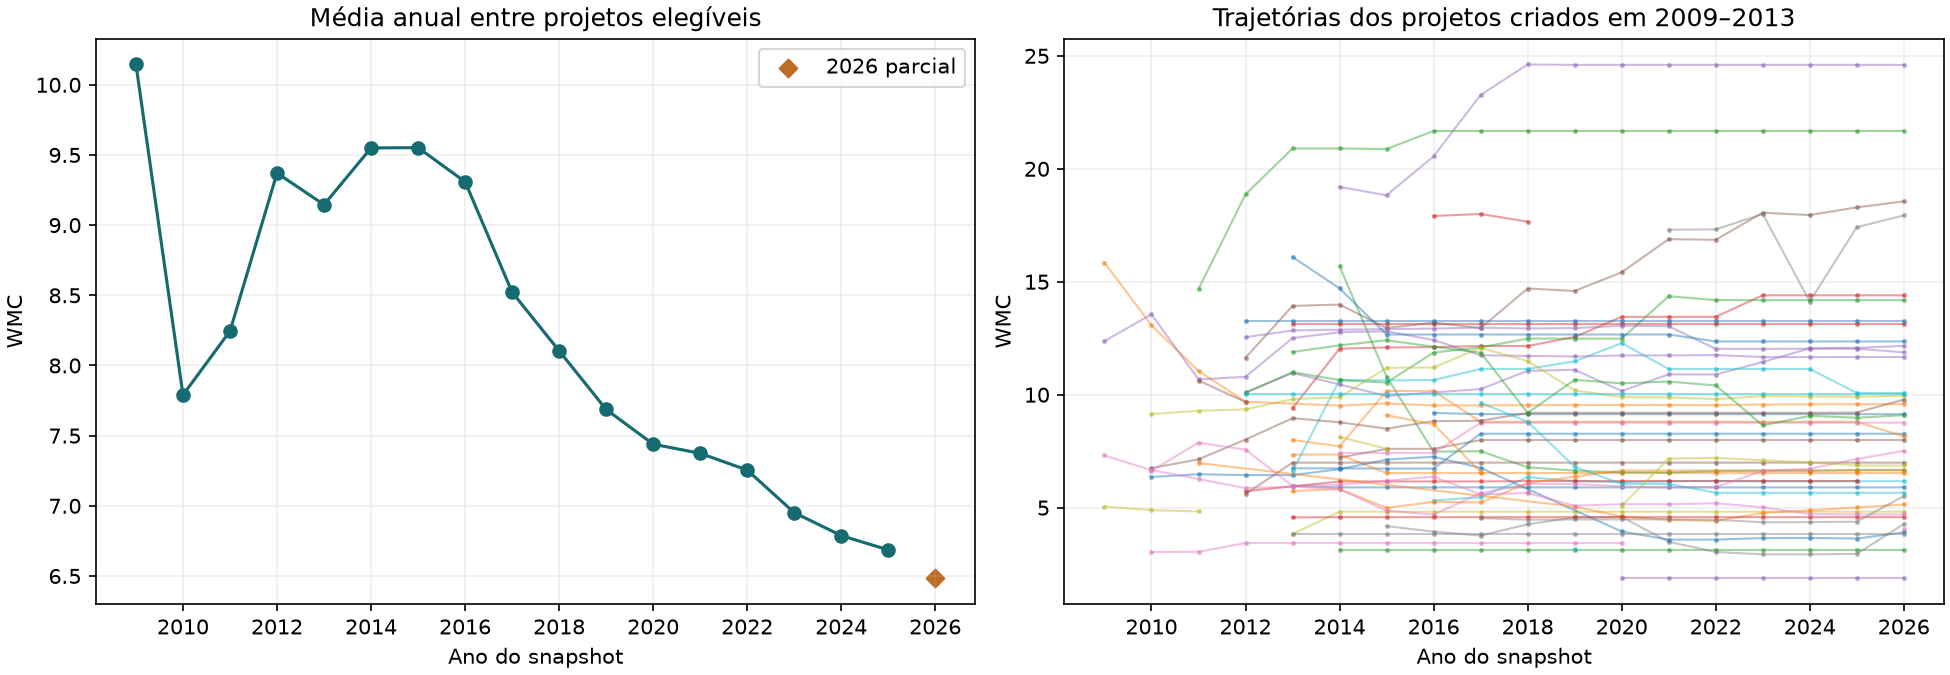
\includegraphics[width=\linewidth]{../Instrumentos/Codigos/Artefatos/evolucao_spring/runs/20261011_historico_v3/figures/avg_wmc.png}
\caption{WMC no histórico: mediana anual dos elegíveis de todas as coortes (esquerda) e trajetórias individuais da coorte antiga (direita). O período de 2026 é parcial. Mudanças da composição afetam as medianas anuais.}
\label{fig:historico-wmc}
\end{figure}

\subsection{Mudanças que acompanharam Spring Boot}

Na coorte antiga, 16 projetos possuem versões elegíveis antes e depois da primeira presença anual observável de Boot, em anos completos. A Tabela~\ref{tab:historico-boot} mostra medianas antes/depois e, separadamente, a mediana das diferenças calculadas projeto a projeto. Essa última não equivale à subtração das duas medianas marginais.

\begin{table}[htbp]
\centering\small
\caption{Spring Boot na coorte antiga: mesmos 16 projetos antes e depois ($n_a=n_b=16$).}
\label{tab:historico-boot}
\begin{tabular}{lrrr}
\hline
Métrica & Mediana antes & Mediana depois & Mediana das diferenças \\
\hline
CBO & 5,437 & 5,516 & 0,0686 \\
RFC & 9,553 & 9,819 & -0,0326 \\
WMC & 10,027 & 10,121 & -0,2760 \\
LOC/método & 6,079 & 6,166 & -0,1897 \\
DIT & 1,356 & 1,297 & -0,0016 \\
NOC & 0,076 & 0,069 & -0,0005 \\
LCOM* & 0,290 & 0,301 & 0,0001 \\
\hline
\end{tabular}
\end{table}

A mediana das mudanças é positiva para CBO e próxima de zero para LCOM*, e negativa para RFC, WMC, LOC por método, DIT e NOC. As magnitudes descrevem esta amostra; não são testes de significância ou efeitos causais. Quatorze pares usam anos consecutivos, um tem intervalo de dois anos e o Causeway tem intervalo de oito anos entre versões elegíveis. Esse último agrega muitas mudanças concorrentes. No conjunto das quatro coortes, existem 21 pares completos de Boot. As tabelas de contexto preservam separadamente os projetos sem transição observada nas mesmas janelas.

Também há Boot preliminar antes de 2014: o snapshot de 2013 de \texttt{spring-guides/gs-rest-service} declara 0.5.0.M6. Com 43 LOC, ele fica fora da comparação principal, mas permanece registrado. Isso não contradiz o lançamento estável de abril de 2014.

\subsection{Mudanças que acompanharam evidências de IA}

Onze projetos antigos apresentam evidência em alguma versão elegível. Apenas um possui par em anos completos até 2025: OpenESPI-DataCustodian, de 2024 para 2025. A evidência de coautoria Claude foi integrada em 1º de julho de 2025; a data de autoria é 24 de junho. No mesmo ano aparece Boot, impedindo separar essas mudanças. CBO passa de 9,895 para 12,180 e WMC de 11,140 para 10,079. Esse caso isolado não representa o comportamento geral de projetos assistidos por IA.

Os outros dez pares antigos usam 2025 e o corte parcial de 2026, fixado em 11 de outubro de 2026 às 19:34:13 UTC. A Tabela~\ref{tab:historico-ia-parcial} mantém esse acompanhamento separado. Sinais como identidades de bot, arquivos de instruções e entradas de gitignore não determinam quanto código foi gerado nem demonstram uso contínuo.

\begin{table}[htbp]
\centering\small
\caption{IA na coorte antiga: dez pares com acompanhamento parcial em 2026 ($n_a=n_b=10$).}
\label{tab:historico-ia-parcial}
\begin{tabular}{lrrr}
\hline
Métrica & Mediana antes & Mediana parcial & Mediana das diferenças \\
\hline
CBO & 5,542 & 5,634 & 0,0267 \\
RFC & 9,977 & 10,119 & 0,2813 \\
WMC & 6,082 & 6,515 & 0,2008 \\
LOC/método & 6,619 & 6,710 & 0,0249 \\
DIT & 1,399 & 1,394 & -0,0001 \\
NOC & 0,119 & 0,135 & -0,0009 \\
LCOM* & 0,229 & 0,232 & 0,0024 \\
\hline
\end{tabular}
\end{table}

Na amostra de todas as coortes, há quatro pares de IA em anos completos e 17 pares adicionais no período parcial. As contagens são menores que o total de positivos porque nem todo projeto tem uma versão anterior elegível sem evidência. Esses resultados permitem descrever os casos, mas não sustentar uma conclusão geral de melhora ou piora associada à IA. A ausência dos sinais procurados também não estabelece um grupo comprovadamente sem uso.

\subsection{Síntese das evidências e limites}

O estudo recuperou trajetórias e mudanças estruturais de projetos antigos, incluindo inativos e arquivados que a seleção anterior excluía. A hipótese de progresso uniforme da comunidade não é sustentada por essas descrições: as métricas têm direções distintas, há estabilidade por inatividade e as amostras anuais mudam. Os pares de Boot mostram mudanças observáveis, enquanto o acompanhamento de IA é recente e reduzido. Tamanho, idade, domínio, composição da equipe e migração de framework permanecem explicações concorrentes.

A amostra vem de metadados atuais e a identificação técnica depende de declarações reconhecidas. Projetos com configurações antigas em Ant, dependências dinâmicas ou versões não resolvidas podem permanecer não confirmados. Os resultados não estimam a evolução de toda a comunidade Java nem medem produtividade, desempenho de execução ou funcionalidade. As tabelas de produção e testes, as janelas de comparação e os diagnósticos devem acompanhar a interpretação dos valores agregados. O relatório histórico é descritivo, sem p-valores, deltas de Cliff ou nota única de maturidade.


\subsection{Papel dos resultados transversais anteriores}

O piloto inicial de outubro de 2026 mediu 50 candidatos com classificação disponível: 16 com vestígios e 34 sem evidência detectada. Somente 19 satisfizeram a comparação principal daquela execução, sendo quatro positivos e 15 sem sinais. O piloto ampliado percorreu 1.520 candidatos da seleção anterior e reteve 879, dos quais 187 positivos e 692 sem evidência. Esses números descrevem seleções e instrumentos diferentes da execução histórica.

Na ampliação transversal, RFC, WMC e LOC por método apresentaram medianas maiores no grupo com evidências de IA. Os projetos desse grupo também eram maiores: mediana de 17.445 LOC, contra 7.434. Os contrastes eram sensíveis ao recorte, e a seleção favorecia popularidade e atividade recente. O código medido era atual, inclusive para projetos criados em E1; esses resultados não demonstram o efeito de IA nem a evolução do código desde 2009. O detalhamento, incluindo os testes originalmente calculados, permanece nos arquivos de reprodução e em \texttt{Artigo/Arquivo}.


\bibliographystyle{sbc}
\bibliography{sbc-template}

\appendix
\section*{Apêndice A --- Visualizações históricas e leitura dos resultados}
\label{ap:visualizacoes}

Os gráficos de trajetória usam o ano do snapshot no eixo horizontal e uma medida CK por painel. São apresentadas separadamente a mediana anual entre projetos e as linhas individuais dos projetos criados entre 2009 e 2013. O ponto parcial de 2026 é identificado; lacunas de cobertura não são substituídas por zero. Mudanças na mediana anual podem decorrer da composição de projetos disponíveis, enquanto a trajetória individual acompanha o mesmo repositório.

As tabelas por época apresentam uma contribuição por repositório, com quantidades de projetos e snapshots. O total de projetos únicos não deve ser obtido pela soma das épocas, pois um mesmo projeto pode atravessá-las. Os contrastes por evidência distinguem presença observada, ausência de evidência e transição dentro da época.

Nas tabelas antes/depois, \texttt{n\_a} é o número de projetos com medição anterior e \texttt{n\_b} o número com medição posterior. Os pares correspondem aos mesmos repositórios. A diferença é calculada dentro de cada par antes de obter a mediana; ela não precisa coincidir com a subtração entre as medianas dos dois lados. Os SHA e as datas permitem conferir cada versão utilizada.

As sete medidas conservam suas unidades originais. Não se cria uma nota composta de maturidade. Não se apresentam p-valores, deltas de Cliff ou afirmações automáticas de melhoria. Arquivos CSV, gráficos PNG/SVG, referências fixadas, evidências, diagnósticos e hashes do instrumento integram o pacote de reprodução. Os relatórios dos pilotos transversais anteriores permanecem identificados separadamente.


\end{document}
